\subsection{Classifieur histogramme radial}
\subsubsection{État de l'art}
Cette technique avait été utilisée avec succès pour la reconnaissance de signes de la main avec une caméra Kinect\cite{matthewTang}, c'est pourquoi nous avons jugé intéressant de l'implémenter.

\subsubsection{Présentation de la méthode}

Cette méthode de classification consiste à extraire comme vecteur caractéristique de la main un histogramme radial pondéré des pixels de la main autour d'un centre, pour ensuite classifier ce vecteur à l'aide de classifieurs Bayésiens, $K$ plus proches voisins ou réseau de neurone à une couche cachée.

\paragraph{Calcul de l'histogramme radial}
Intuitivement, l'histogramme radial consiste à calculer un histogramme de projection des pixels de la main "autour" du centre de gravité de la main. Pour déterminer celui-ci, définissons tout d'abord $I$ l'image de la main segmentée et binarisée:

\[
I(x,y) = \left\{
  \begin{array}{l l}
    1 & \quad \text{si $(x,y)$ est un pixel de la main}\\
    0 & \quad \text{sinon}
  \end{array} \right.
\]

Nous déterminons ensuite une image $I'$ de décalage d'angles, qui associe, pour chaque droite passant par le centre de gravité $c = (x_c, y_c)$ de la main, un niveau de gris distinct. C'est en calculant l'histogramme des niveaux de gris de cette image que nous obtenons l'histogramme radial. Ainsi, nous définissons $I'$ de la façon suivante pour tout $(x,y)$ de la main:

\[
I'(x,y) = tan^{-1}(\frac{x - x_c}{y - y_c})
\]

\begin{figure}[htb!]
\centerline{
\includegraphics{handAngleOffsets.png}}
\caption{Image de décalages d'angles}
\label{fig:decalageAngles}
\end{figure}

Nous calculons alors l'histogramme des niveaux de gris de cette image, et nous obtenons alors des histogrammes donnant des pics distincts pour chaque doigt de la main (\autoref{fig:histoRadialGravite}). Il est important de noter que l'histogramme radial est invariant par rotation de centre le centre de gravité et d'angle $\pi$, ce qui nous permet de classifier la main même lorsqu'elle se retrouve à pointer vers le bas après redressement.

\begin{figure}[htb!]
\centerline{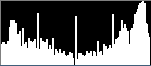
\includegraphics{handMassRadialHist.png}}
\caption{Histogramme radial avec centre de gravité.}
\label{fig:histoRadialGravite}
\end{figure}

Cependant, le centre de gravité a tendance à être positionné là où le pouce et l'auriculaire ont le même niveau de gris dans l'image de décalages d'angles. C'est pourquoi nous utilisons à la place du centre de gravité de la main le centre de la paume de la main. Celui-ci étant placé plus bas sur la main, celui-ci produit des pics plus distincts pour chaque doigt dans l'histogramme radial (\autoref{fig:histoRadialPaume}).

\begin{figure}[htb!]
\centerline{
\includegraphics{handPalmRadialHist.png}}
\caption{Histogramme radial avec centre de la paume)}
\label{fig:histoRadialPaume}
\end{figure}

L'histogramme radial ainsi obtenu constitue le vecteur caractéristique de la main. Nous avons utilisé plusieurs méthodes pour classifier ce vecteur caractéristique:

\begin{itemize}
\item Classifieur Bayésien simple, sans spécificité particulière. Nous avons pour cela utilisé la classe CvNormalBayesClassifier du module machine learning d'OpenCV.
\item $K$ plus proches voisins, encore une fois sans spécificités. Nous avons pour cela utilisé la classe CvKNearestClassifier du module machine learning d'OpenCV.
\item Réseau de neurones artificiels, avec une topologie à $3$ couche:

\begin{itemize}
\item Une couche d'entrée avec $n$ neurones, correspondants aux $n$ classes de l'histogramme radial.
\item Une couche cachée avec $k$ neurones, où $k$ est variable selon le compromis précision/efficience souhaité.
\item Une couche de sortie avec $m$ neurones, où $m$ est le nombre de classes dans lesquelles nous souhaitons classifier l'histogramme (généralement 6, une pour chaque nombre de doigts possibles). La valeur maximale du vecteur de sortie correspond à la classe choisie.
\end{itemize}
\end{itemize}

\paragraph{Calcul de sous-classes automatique par $K$ moyennes}
Un problème rencontré est que des images de mains comportant le même nombre de doigts peuvent avoir des histogrammes radiaux très différent. Cela est du entre autre au nombre de façon différentes de lever 3 doigts, par exemple. Cela pose problème dans le cadre du classifieur Bayésien et du classifieur avec réseaux de neurones. Pour ceci, nous avons évalué plusieurs approches:

\begin{itemize}
\item Séparer chaque classe en sous-classe, de telle façon à ce que chaque sous-classe corresponde à une configuration de la main donnée. Ainsi, nous obtenons 32 classes distinctes (1 bit pour chaque doigt). Cette méthode s'est prouvée infructueuse étant donné le manque de données d'apprentissage pour la plupart des configurations de doigts.
\item Utiliser un algorithme d'apprentissage non supervisé pour classer les histogrammes radiaux de mains de la base d'apprentissage ayant le même nombre de doigts dans des sous-classes d'histogrammes radiaux proches. Cette deuxième approche s'est montrée efficace pour augmenter le taux de reconnaissance avec le classifieur Bayésien.
\end{itemize}

\subsubsection{Analyse des résultats}
\paragraph{Mesure du taux de reconnaissance}
Étant donné la petite taille des données disponibles, il n'a pas été fructueux de séparer les images dans une base d'apprentissage (servant à entraîner les classifieurs Bayésiens, KPPV et réseau de neurone) et une base de test (servant à mesurer le taux de reconnaissance) uniques et distinctes. Nous avons résolu le problème en mesurant le taux de reconnaissance par la méthode du "leave one out":

Soit $Q = \{(image, nbdoigts), ...\}$ une base contenant toutes les images disponibles.
\begin{itemize}
\item Initialiser une variable $c$ à 0.
\item Pour chaque $q_i = (image_i, nb_i) \in Q$, faire:
\begin{itemize}
\item Utiliser $Q - \{q_i\}$ comme base d'apprentissage pour le classifieur
\item Si le classifieur retourne $nb_i$ pour $image_i$, alors incrémenter $c$
\end{itemize}
\item Le taux de reconnaissance est alors $\frac{c}{|Q|}$
\end{itemize}

C'est par cette méthode que le taux de reconnaissance est mesuré dans les paragraphes suivants.

\paragraph{Classifieur Bayésien et choix du nombre de classes pour l'histogramme}
Un paramètre important est le choix du nombre de classes pour l'histogramme radial de la main. Pour cela, nous avons mesuré le taux de reconnaissance en fonction du nombre de classes de l'histogramme avec le classifieur Bayésien, qui ne nécessite pas de paramètres supplémentaires.

\begin{figure}[htb!]
\centerline{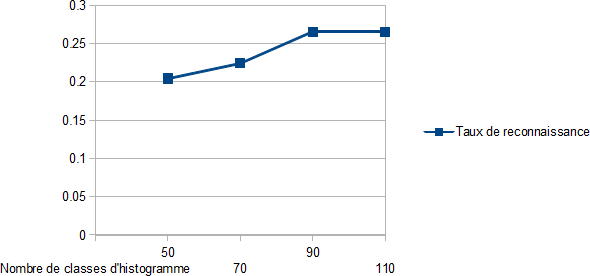
\includegraphics[scale=0.8]{bayesRate.png}}
\caption{Taux de reconnaissance par rapport au nombre de classes de l'histogramme avec classifieur de Bayes.}
\label{fig:bayesRates}
\end{figure}

Le taux de reconnaissance croît avec le nombre de classes de l'histogramme, jusqu'à atteindre un plafond à $90$ classes d'histogramme environ (\autoref{fig:bayesRates}). Ajouter des sous-classes calculées avec l'algorithme des $K$ moyennes permet d'augmenter sensiblement ce taux (\autoref{fig:bayesRates2}). Cependant cela rajoute un élément aléatoire, lié à l'initialisation des sous-classes.

\begin{figure}[htb!]
\centerline{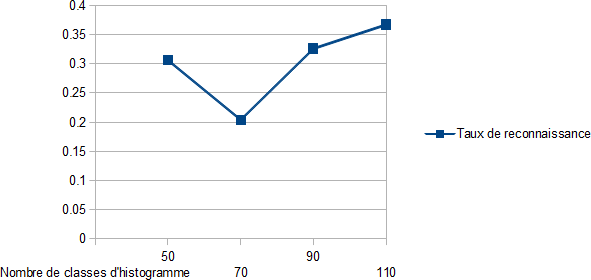
\includegraphics[scale=0.8]{bayesRates2.png}}
\caption{Taux de reconnaissance par rapport au nombre de classes de l'histogramme avec $2$ sous-classes par classe.}
\label{fig:bayesRates2}
\end{figure}

\paragraph{Classifieur $K$ plus proches voisins}
En fixant le nombre de classes de l'histogramme à $90$, et en faisant varier $K$, nous obtenons un taux de reconnaissance maximal de $38$\% avec $K = 7$ (\autoref{fig:kppvRates}).

\begin{figure}[htb!]
\centerline{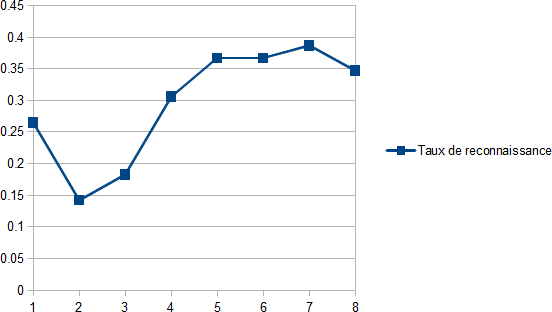
\includegraphics[scale=0.8]{kppvRates.png}}
\caption{Taux de reconnaissance par rapport à $K$ avec les $K$ plus proches voisins}
\label{fig:kppvRates}
\end{figure}

\paragraph{Classifieur avec réseau de neurones artificiels}
En fixant de nouveau le nombre de classes de l'histogramme à $90$, et en faisant varier le nombre de neurones de l'unique couche cachée, nous obtenons un taux de reconnaissance maximal de $26$\%  avec $450$ neurones dans la couche cachée. Il semble difficile d'obtenir un taux de reconnaissance supérieur à un choix aléatoire uniforme (\autoref{fig:annRates}).

\begin{figure}[htb!]
\centerline{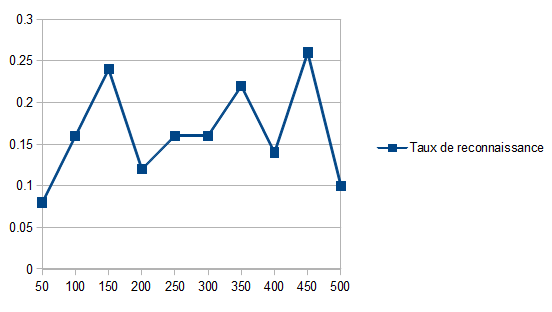
\includegraphics[scale=0.8]{ANNRates.png}}
\caption{Taux de reconnaissance par rapport au nombre de neurones dans la couche cachée}
\label{fig:annRates}
\end{figure}

\paragraph{Conclusion, problèmes et améliorations possibles}
Après mesure des résultats, nous avons décidé d'utiliser le classifieur avec $K$ plus proches voisins car celui-ci offre à la fois le meilleur taux de reconnaissance et les meilleures performances en terme de temps de calcul. Cependant, le taux de reconnaissance n'atteint que 38\%, ce qui montre plusieurs problèmes avec cette approche:
\begin{itemize}
\item Malgré le redressement de l'image, certaines images sont mal redressées et sont donc mal classifiées.
\item Comme les pics abrupts le montre sur (\autoref{fig:histoRadialPaume}), cette méthode est sensible au bruit dans l'image, et également à la présence ou non du poignet après la segmentation.
\item Le nombre d'image disponibles pour effectuer l'apprentissage est limité, et toutes les configurations de doigts ne sont pas représentées ou seulement une fois. On peut raisonnablement espérer un meilleur taux de reconnaissance avec une plus grande base d'apprentissage.
\end{itemize}